\documentclass[10pt,twocolumn]{article}
\usepackage[margin=0.62in]{geometry}
\usepackage{graphicx}
\usepackage{booktabs}
\usepackage{amsmath,amssymb,bm}
\usepackage{microtype}
\usepackage[font=small,labelfont=bf]{caption}
\usepackage{enumitem}
\usepackage{titlesec}
\usepackage{url}
\setlength{\columnsep}{0.24in}
\setlength{\parindent}{1em}
\setlength{\parskip}{0pt}
\setlength{\textfloatsep}{6pt plus 2pt minus 2pt}
\setlength{\intextsep}{5pt plus 1pt minus 1pt}
\setlength{\floatsep}{5pt plus 1pt minus 1pt}
\setlength{\abovedisplayskip}{3pt plus 1pt minus 1pt}
\setlength{\belowdisplayskip}{3pt plus 1pt minus 1pt}
\setlist[itemize]{leftmargin=1.2em,itemsep=1pt,topsep=2pt,parsep=0pt}
\titlespacing*{\section}{0pt}{5pt}{2pt}
\titlespacing*{\subsection}{0pt}{4pt}{1pt}
\captionsetup{skip=3pt}

\title{\vspace{-1.4em}\bfseries Learning Topological Phases from Quantum Geometry\\[-1pt]
\large Midway 1 Progress Report}
\author{Rajat Shuvra Saha\\[-1pt]\normalsize National Institute of Science Education and Research, Bhubaneswar}
\date{October 2026}

\begin{document}
\maketitle
\vspace{-1.2em}

\begin{abstract}
Topological invariants describe global properties of occupied bands, whereas quantum geometry provides momentum-resolved information about Bloch states. This report presents a physics-informed learning pipeline for a two-band Hamiltonian family. The code generates synthetic Hamiltonians, computes exact quantum-geometric targets and Chern labels, and forms a 19-channel input tensor for a local--global neural network. The network reconstructs four quantum-geometric fields and classifies the Chern number. In the current run, a 141-point Qi--Wu--Zhang (QWZ) mass scan gives a classifier accuracy of 0.466 and macro-F1 of 0.274; integrated predicted curvature also has substantial error. A validation-loss bookkeeping issue currently causes epoch-one checkpoint selection, so these numbers are preliminary and must be recomputed after fixing model selection.
\end{abstract}

\section{Introduction}
A Chern number is a global invariant obtained by integrating Berry curvature over the Brillouin zone (BZ). This work asks whether a neural network can infer global topology from local quantum-geometric structure while reconstructing interpretable intermediate fields. The present stage is a controlled synthetic experiment; training examples are generated by the code rather than loaded from an existing dataset.

\section{Related Work}
The Qi--Wu--Zhang lattice Hamiltonian is a standard minimal Chern-insulator benchmark with analytically known phase boundaries \cite{qi2006}. Berry curvature describes the geometric phase accumulated by quantum states as parameters vary \cite{berry1984}. Here these established ingredients are combined in a supervised, physics-informed model that predicts both local QGT fields and a global Chern class; no external QWZ dataset is used.

\section{Method}
The two-band Hamiltonian is written as
\begin{equation}
H(\mathbf{k})=\mathbf{d}(\mathbf{k})\cdot\boldsymbol{\sigma},\qquad
\hat{\mathbf d}=\frac{\mathbf d}{|\mathbf d|}.
\label{eq:h}
\end{equation}
For the lower band, the exact quantum metric and Berry curvature are computed from analytic derivatives:
\begin{align}
g_{\mu\nu}(\mathbf{k})&=\frac14\,\partial_\mu\hat{\mathbf d}\cdot\partial_\nu\hat{\mathbf d},\label{eq:metric}\\
\Omega_{xy}(\mathbf{k})&=-\frac12\,\hat{\mathbf d}\cdot\left(\partial_x\hat{\mathbf d}\times\partial_y\hat{\mathbf d}\right),\\
C&=\frac{1}{2\pi}\int_{\mathrm{BZ}}\Omega_{xy}(\mathbf{k})\,d^2k.
\label{eq:chern}
\end{align}

\textbf{Input and outputs.} The ML input is \emph{not} the QGT itself. It is a $19\times N_k\times N_k$ tensor containing $\mathbf d$ (3 channels), $\hat{\mathbf d}$ (3), $\partial_x\hat{\mathbf d}$ (3), $\partial_y\hat{\mathbf d}$ (3), $\nabla^2\hat{\mathbf d}$ (3), $|\mathbf d|$, $1/|\mathbf d|$, and the two gradient magnitudes. With $N_k=40$, each input has shape $19\times40\times40$. The targets are
\begin{equation}
Y=\left[\log(1+g_{xx}),\ g_{xy},\ \log(1+g_{yy}),\ \operatorname{Im}Q_{xy}\right],
\end{equation}
plus a class label $C\in\{-1,0,+1\}$. The network, \texttt{PhysicsQGTNet}, combines a high-resolution local branch, a multi-scale periodic U-Net and an attention-pooled global classifier. It returns a $4\times40\times40$ field estimate and three Chern-class logits. Berry curvature is decoded as $\widehat\Omega_{xy}=-2\operatorname{Im}\widehat Q_{xy}$.

\begin{figure}[t]
\centering
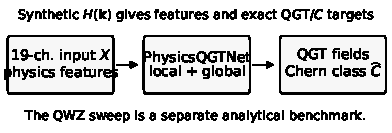
\includegraphics[width=\columnwidth]{figures/workflow.pdf}
\caption{Current workflow. Physics routines generate input features and exact targets; learning occurs in the shared local--global network.}
\label{fig:workflow}
\end{figure}

The composite training objective is
\begin{equation}
\mathcal L=4\mathcal L_{\mathrm{QGT}}+\mathcal L_{\mathrm{geom}}+2\mathcal L_{\mathrm{topo}}+0.5\mathcal L_{\mathrm{cls}},
\end{equation}
where the terms penalize field reconstruction error, violation of the two-band identity $g_{xx}g_{yy}-g_{xy}^2=\Omega_{xy}^2/4$, disagreement between integrated predicted curvature and the Chern label, and classification error. The geometric identity is used only for this two-band pure-state model.

\section{Dataset and Experimental Setup}
Training/validation samples are generated on a periodic $40\times40$ BZ from randomized generalized two-band Hamiltonians. Samples are grouped into the three Chern classes, with 300 examples per class for training (900 total) and 75 per class for validation (225 total). The generator rejects near-gap-closing examples; the realised training set has a minimum gap of about $0.401$ in the code's energy units. Training uses batch size 12, 100 epochs, AdamW with learning rate $10^{-3}$ and weight decay $10^{-4}$. The benchmark sweep uses 141 QWZ mass values over $[-3.5,3.5]$, excluding near-gapless parameter values rejected by the minimum-gap cutoff. No external materials database is used in this stage.

\section{Results}
The QWZ Hamiltonian is
\begin{equation}
H_{\mathrm{QWZ}}=\sin k_x\,\sigma_x+\sin k_y\,\sigma_y+(m+\cos k_x+\cos k_y)\sigma_z,
\end{equation}
with analytical lower-band phases $C=0$ for $m<-2$ and $m>2$, $C=+1$ for $-2<m<0$, and $C=-1$ for $0<m<2$. Figure~\ref{fig:qwz} compares this reference with the current model predictions. Quantitative metrics from the notebook are summarised in Table~\ref{tab:results}.

\begin{table}[t]
\centering
\caption{Current QWZ benchmark metrics.}
\label{tab:results}
\small
\begin{tabular}{lr}
\toprule
Metric & Current run \\
\midrule
Classifier accuracy & 0.4661 \\
Macro-F1 & 0.2744 \\
Integrated-Chern MAE & 0.7331 \\
Integrated-Chern RMSE & 0.9354 \\
Mean four-field QGT RMSE & 0.2987 \\
\bottomrule
\end{tabular}
\end{table}

\begin{figure}[t]
\centering
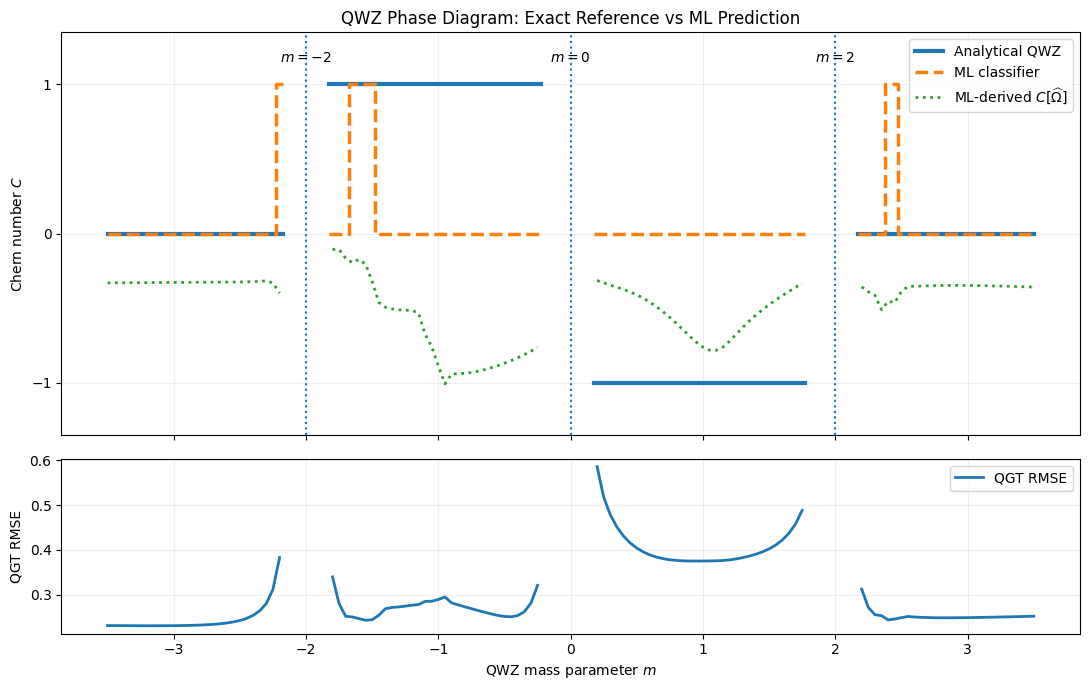
\includegraphics[width=\columnwidth]{figures/qwz_phase_diagram.png}
\caption{Notebook output for the QWZ scan: analytical phase reference, predicted class, Chern number from integrated predicted curvature, and field RMSE. The current predictions do not reliably recover the phase plateaus.}
\label{fig:qwz}
\end{figure}

For one unseen synthetic Hamiltonian, the exact class is $C=0$ and the classifier also predicts $0$, but integrating its predicted curvature gives $C[\widehat\Omega]=-0.325$ (the exact numerical integral is approximately zero). The minimum gap is $2.452$. The corresponding Berry-curvature maps in Fig.~\ref{fig:omega} show that the local reconstructed field is not yet quantitatively reliable.

\begin{figure}[t]
\centering
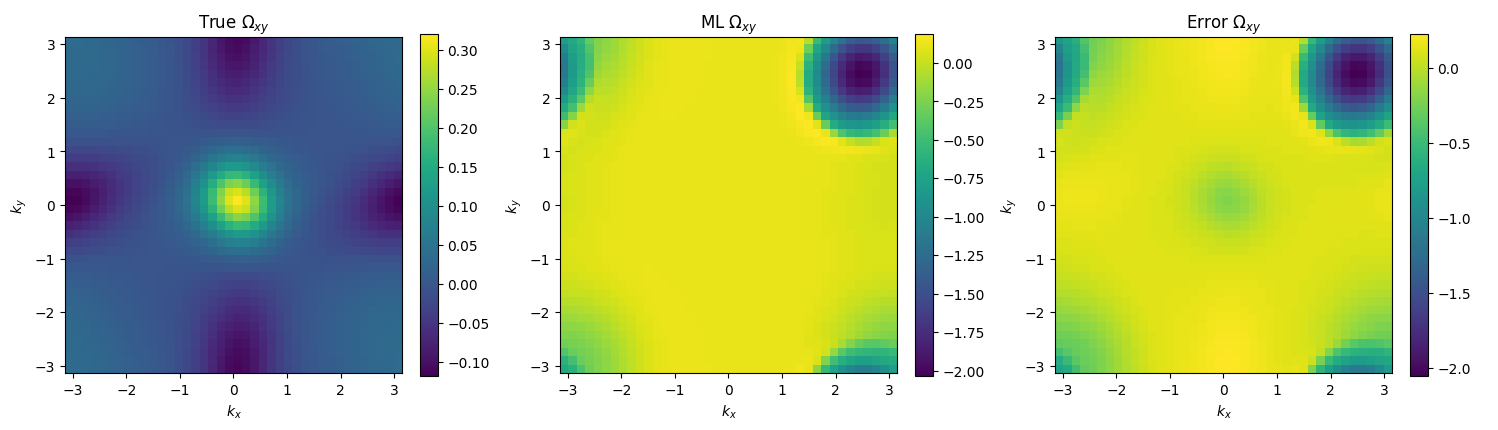
\includegraphics[width=\columnwidth]{figures/berry_curvature_reconstruction.png}
\caption{Berry curvature for one unseen synthetic sample: exact field, ML prediction and pointwise error. The mismatch explains why agreement of the classifier on this one example does not establish accurate geometric reconstruction.}
\label{fig:omega}
\end{figure}

\begin{figure}[t]
\centering
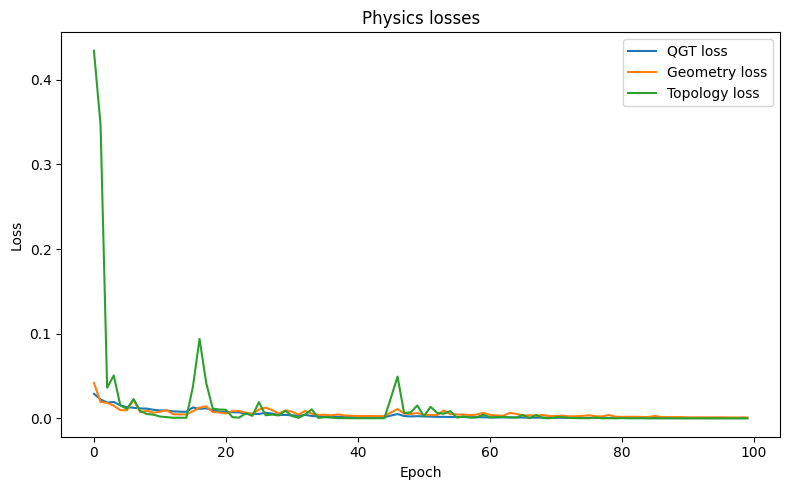
\includegraphics[width=0.96\columnwidth,height=1.30in,keepaspectratio]{figures/physics_losses.png}
\caption{Validation components during the 100-epoch run. Component losses decrease, but checkpoint selection is invalidated by the total-loss bookkeeping issue discussed below.}
\label{fig:loss}
\end{figure}

\section{Analysis and Limitations}
The current results are a baseline, not evidence of successful phase-diagram recovery. The QWZ classification accuracy (0.466) and macro-F1 (0.274) are low, while the curvature-integrated Chern errors are appreciable. The single unseen sample shows that the class head and curvature-integral route can disagree. These results motivate further checks of field normalisation, feature scaling, class generalisation and performance near phase boundaries.

A code issue must be fixed before interpreting the run as a converged model: \texttt{evaluate()} accumulates a key named \texttt{loss}, but \texttt{physics\_loss()} returns the total under \texttt{total}. The reported validation total therefore remains zero, and the best-checkpoint logic selects epoch 1. Consequently, benchmark numbers above are from that selected checkpoint, not a correctly selected final model. The immediate next step is to correct the key consistently, retrain, and regenerate the phase diagram and metrics.

\section{Conclusion}
A complete synthetic data-generation and multi-task learning pipeline is implemented, including exact two-band QGT targets, a 19-channel local input, QGT reconstruction and three-class Chern prediction. The QWZ sweep currently exposes substantial generalisation error rather than confirming transfer. After fixing checkpoint selection, the benchmark should be repeated before progressing to spinful Kane--Mele and later JARVIS--Wannier Hamiltonians.

\section*{Acknowledgements}
The reported dataset is generated by the project code using NumPy and PyTorch. No external material database contributes to these results; JARVIS--Wannier testing remains future work.

\begin{thebibliography}{9}
\setlength{\itemsep}{0pt}
\bibitem{qi2006} X.-L. Qi, Y.-S. Wu, and S.-C. Zhang, ``Topological quantization of the spin Hall effect in two-dimensional paramagnetic semiconductors,'' \textit{Phys. Rev. B} \textbf{74}, 085308 (2006).
\bibitem{berry1984} M. V. Berry, ``Quantal phase factors accompanying adiabatic changes,'' \textit{Proc. R. Soc. A} \textbf{392}, 45--57 (1984).
\end{thebibliography}

\end{document}
